
\section{COCOMO vs Other}\label{sect:other}

What if you do not have access to projects
expressed using the COCOMO attributes?
As
discussed on this section, it is possible
to achieve results competitive
to COCOMO, by other means.

This section presents results where the {\em same} projects
were expressed in two sets of attributes:
\bi
\item The COCOMO attributes of \fig{parems};
\item Some NASA-specific terminology.
\ie
To these projects, we apply COCOMO (on the COCOMO attributes)
and a non-parametric method to the remaining attributes
These experiments go somewhat beyond 
That said, not that the results in this section 
{\em do not} say that be

  can be reached by other methods.

Our first experiment comments on 
a frequent comment made when we disucss this
work with our colleageues. When we report
that old COCOMO does better than


 
Experiment \#1 shows that, at least on some NASA data,
recent state-of-the-art effort estimations methods
perform no better than a decade old COCOMO model.
This result motivates the more extensive studies, reported later in this paper.

Experiment \#1 compares COCOMO-II with a 
case-based reasoning (CBR) method.
CBR matches details  of a current
project to a library of past completed projects. Decisions about the
current project are made by reflecting over similar 
prior completed projects~\cite{schank77a,kol93}.
CBR does not build an intermediary model of
(e.g.) the correlation between lines of code and defects. Rather,
all reasoning is a partial match between the new examples and the old
examples.



State-of-the-art CBR tools such 
use a variety of techniques to handle
noisy data, outliers, and irrelevant attributes.
For example, the WHERE tool of Menzies et al.~\cite{me11m}
recursively divides the cases using dimensions
synthesized by a 
principle component analysis\footnote{For reasons of efficiency, {\em WHERE}
  uses the $O(2N)$ FASTMAP
  method~\cite{platt05,Faloutsos1995} rather than
  the standard $O(N^2)$ method to find these
  principle components~\cite{Du2008}.} that filters out irrelevant attributes.

WHERE is a {\em prototype learner}~\cite{chang74}
 that replaces $N$ examples with $M \ll N$ most informative prototypes.
To find those prototypes, 
WHERE's recursive descent returns on set of related cases.
For each such set, WHERE generates one centroid representing the median values
of each division. 
Prototype learners like WHERE  are known to mitigate for data outliers since 
noisy outliers disappear from the prototypes~\cite{chang74}.


Those prototypes can be used for effort estimation. 
The SLOPE algorithm of Papakroni~\cite{papa13} is
a non-parametric response surface method that generates estimates for a project by
 interpolating between
the two nearest centroids (found by WHERE).  This interpolation is weighted by the
distance to each centroid (and the estimate from
the closer centroid has more weight, see \fig{slope}).
\begin{figure}[!t]
\begin{lstlisting}
def SLOPE(data,project):
   prototypes= WHERE(data)
   neighbors = distances(project,prototypes) 
   one, two  = neighbors[0],neighbors[1] #two closest
   d1, d2    = dist(one,project), dist(two,project)
   w1, w2    = 1 /d1,  1 /d2 #closest has most weight
   est1, est2= effort(one), effort(two)
   return (w1*est1 + w2*est2) / (w1 + w2) 
\end{lstlisting}
\caption{SLOPE: a non-parametric response surface method that 
generates estimates from a  set of piecewise linear approximations.}\label{fig:slope}
\end{figure}
In an extensive study,
Papakroni~\cite{papa13} found:
\bi
\item For {\em defect prediction}, SLOPE is competitive
with random forests and  Naive Bayes;
\item For {\em effort estimation}, SLOPE is also competitive with
regression trees and linear regression.
\ei
%XXX only the JPL attributes
Papakroni did not compare SLOPE against COCOMO-II.
Accordingly, for this paper, we ran that comparisons
using the extended NASA10  dataset (shown in \fig{types}).
These  17 projects,  dating up to 2010, are described in terms of both:
\bi
\item
The COCOMO-II attributes of
\fig{cparems}
\item
Some domain-specific NASA descriptors.
\ei
For examples of the latter,  at the NASA,  projects are discussed in terms of their development language
and mission type (one of ``observatory'', ``rover'', ``deep space satellite'', etc.
For this study, SLOPE used just the NASA project descriptors and
COCOMO-II used just the COCOMO attributes. 

\fig{mmre} shows the results of that comparison.
%% XXX need to list all the data set
These are ``leave-one-out'' results; i.e. for every project, SLOPE 
were trained on all other projects.  
As for COCOMO-II, it trained on none of the NASA10 data
(i.e.   no
     local calibration) since COCOMO-II generates its estimates using
     Boehm's tunings derived 1990 to 2000 (note that none of the NASA10
projects were used to generate the COCOMO-II tunings).

The performance measure here is the magnitude
of the relative error (and {\em lower} errors are {\em better}):

{\small
\begin{equation}\label{eq:mre}
\mathit{MRE}= \mathit{abs(predicted - actual)/actual}
\end{equation}}
In \fig{mmre}, the median MRE results for SLOPE and COCOMO-II are 52 and 44 (respectively).
The statistical analysis of \fig{a12}
shows that the SLOPE and COCOMO-II results are indistinguishable. 
\begin{figure}
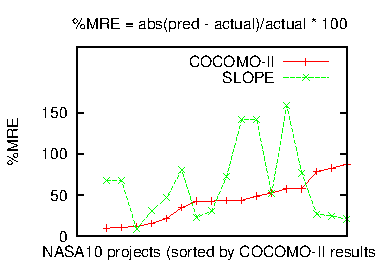
\includegraphics[width=2.5in]{mmre.pdf}
\caption{NASA10 projects; leave-one-out results.
{\em Better} results are {\em lower} on the y-axis.}\label{fig:mmre}
\end{figure}
\begin{figure}[!b]
\small
\begin{tabular}{|p{.95\linewidth}|}\hline
Numerous researchers such as 
Shepperd\&MacDonell~\cite{shepperd12a}; Arcuri\&Briand~\cite{arcuri11}; Kampenes~\cite{kampenes07}  warn that even if an
hypothesis test declares two populations to be
``significantly'' different, then that result is
misleading if the ``effect size'' is very small. For
example, Kocaguenli et al.~\cite{kocharm13} report on the misleading
results of such hypothesis tests in software defect
prediction (due to small size of the effect being
explored).

Hence, to assess 
the performance differences in \fig{mmre}
we first must rule out small effects.
Vargha and Delaney's
non-parametric 
A12 effect size test (recently 
endorsed by Arcuri and Briand
in their ICSE'11 paper~\cite{arcuri11})
explores
two lists $M$ and $N$ of size $m$ and $n$.
A12 computes the probability that numbers in one sample are bigger than in another:
\[A12 = \left(\sum_{x\in M, y \in N} 
\begin{cases} 
1   & \mathit{if}\; x > y\\
0.5 & \mathit{if}\; x == y
\end{cases}\right) / (mn)
\]
For \fig{mmre},  $A12 < 0.6$ 
which is 
Vargha and Delaney's test for recognizing  a ``small'' and negligible effect.
That is, A12 judges that  the differences between the COCOMO-II and SLOPE results
are too small to be of interest.\\\hline
\end{tabular}
\caption{Testing for ``small effects'' using the A12 test.}\label{fig:a12}
\end{figure}


The good news here is that SLOPE (which makes no use
of COCOMO) performs nearly the same as COCOMO-II. This means
that there exists data sets within which it is
possible to be as good as COCOMO, even if we do not
use the COCOMO attributes.

But the more  important result is that the
\mbox{COCOMO-II} results were no worse as those found by SLOPE. This
a startling result since SLOPE made extensive use of the NASA10 data set
(clustering, prototype generation, interpolation between prototypes).
COCOMO-II, on the other hand,  achieved its results without {\em any reflection  on the NASA10 data}.
